\documentclass[11pt,a4paper]{article}
\usepackage[UTF8]{ctex}
\usepackage[margin=2.2cm]{geometry}
\usepackage{graphicx,booktabs,amsmath,amssymb,hyperref,xcolor,listings,float,enumitem,caption,multirow}
\usepackage{tikz}
\usetikzlibrary{shapes.geometric,arrows.meta,positioning,calc,fit,backgrounds}

\hypersetup{colorlinks=true,linkcolor=blue,urlcolor=blue}
\lstset{language=C,basicstyle=\ttfamily\small,keywordstyle=\color{blue}\bfseries,
  commentstyle=\color{gray},numbers=left,numberstyle=\tiny\color{gray},
  breaklines=true,frame=single,tabsize=4,captionpos=b}

\title{\textbf{项目三：C语言高性能矩阵乘法}\\[0.4em]
\large 在 Apple M5 上从 0.69 到 385 GFLOPS —— 558 倍加速}
\author{姓名：闫伦翰 \quad 学号：12412823}
\date{2026年5月}

\begin{document}
\maketitle

\section{引言}

矩阵乘法 $C=A\times B$ 是深度学习的计算核心。
本项目使用 C 语言实现单精度（\texttt{float}）矩阵乘法，
并通过六个优化阶段，在 $8192^2$ 规模下达到 \textbf{385 GFLOPS}
（OpenBLAS 的 75\%），相比朴素基线实现了 \textbf{558 倍}加速。

\textbf{测试平台：}
\begin{itemize}[nosep]
  \item \textbf{本地：} Apple M5 MacBook Air --- 4P+6E 核心，16\,GB 内存
  \item \textbf{云端：} 阿里云 \texttt{g8y.8xlarge} --- 32 核 ARM（倚天 710），122\,GB（用于 64K 测试）
\end{itemize}

\subsection*{代码结构}

项目由三个源文件组成：

\begin{table}[H]\centering
\begin{tabular}{l|l}
\toprule
\textbf{文件} & \textbf{功能} \\
\midrule
\texttt{matrix.h} & 单头文件库：\texttt{Matrix} 结构体及工具函数 \\
                   & （\texttt{matrix\_create}、\texttt{matrix\_free}、\texttt{matrix\_random}、\texttt{matrix\_zero} 等） \\
\texttt{matmul\_plain.c} & 基线 $i$-$j$-$k$ 实现 + 基准测试驱动（\texttt{main}） \\
\texttt{matmul\_improved.c} & 优化的 BLIS 风格实现（NEON SIMD + OpenMP） \\
\bottomrule
\end{tabular}
\end{table}

\noindent\textbf{编译命令（macOS）：}
\begin{lstlisting}[language=bash,numbers=none,basicstyle=\ttfamily\scriptsize]
gcc -O3 -Xpreprocessor -fopenmp -I$(brew --prefix libomp)/include \
    -L$(brew --prefix libomp)/lib -lomp -I$(brew --prefix openblas)/include \
    -L$(brew --prefix openblas)/lib -lopenblas \
    -o benchmark matmul_plain.c matmul_improved.c -lm
\end{lstlisting}

\section{实现}

\subsection{基线：\texttt{matmul\_plain}}

标准 $i$-$j$-$k$ 循环。内层循环以步长 $n$ 访问 \texttt{B[k][j]}，
导致大量缓存缺失。在 $1024^2$ 规模下达到 \textbf{2.0 GFLOPS}，
在 $8192^2$ 规模下仅有 \textbf{0.69 GFLOPS}。

\subsection{优化：\texttt{matmul\_improved} --- 六个阶段}

% ── 路线图流程图 ──
\begin{figure}[H]
\centering
\begin{tikzpicture}[
  phase/.style={rectangle, rounded corners=4pt, draw=black!70, fill=#1,
    minimum width=2.1cm, minimum height=1.4cm, align=center, font=\small\bfseries},
  arr/.style={-{Stealth[length=5pt]}, thick, gray!70},
  res/.style={font=\scriptsize\color{black!60}, align=center}
]
\node[phase=blue!15]   (p1) {阶段1\\循环重排\\+分块};
\node[phase=blue!15,   right=0.4cm of p1] (p2) {阶段2\\B矩阵打包\\+对齐};
\node[phase=violet!15, right=0.4cm of p2] (p3) {阶段3\\NEON SIMD\\$8\times16$ 微核};
\node[phase=violet!15, right=0.4cm of p3] (p4) {阶段4\\A+B面板\\打包};
\node[phase=orange!20, right=0.4cm of p4] (p5) {阶段5\\OpenMP\\10线程};
\node[phase=red!20,    right=0.4cm of p5] (p6) {阶段6\\BLIS分块\\+预取};

\foreach \n/\v in {p1/16.3,p2/27.2,p3/47.8,p4/47.6,p5/309,p6/\textbf{386}} {
  \node[res, below=0.15cm of \n] {\v\,GF};
}
\draw[arr] (p1)--(p2); \draw[arr] (p2)--(p3); \draw[arr] (p3)--(p4);
\draw[arr] (p4)--(p5); \draw[arr] (p5)--(p6);

\node[res, above=0.1cm of p1] {$\times8$};
\node[res, above=0.1cm of p2] {$\times1.7$};
\node[res, above=0.1cm of p3] {$\times1.7$};
\node[res, above=0.1cm of p4] {基础设施};
\node[res, above=0.1cm of p5] {$\times6.5$};
\node[res, above=0.1cm of p6] {$\times1.2$};
\end{tikzpicture}
\caption{优化路线图（$8192^2$ 下的 GFLOPS，相对上一阶段的加速比）。}
\end{figure}

\subsubsection{阶段1：循环重排 + 缓存分块}

\textbf{问题：} $i$-$j$-$k$ 顺序 $\Rightarrow$ B 矩阵以步长 $n$ 访问 $\Rightarrow$ 缓存缺失率 $>50\%$。

\textbf{解决方案：} 将循环重排为 $i$-$k$-$j$（B 和 C 均为步长 1 访问）+ $64\times64$ 分块。

外层循环将矩阵划分为分块：
\begin{lstlisting}[language={},basicstyle=\ttfamily\scriptsize,frame=single,numbers=none]
for ii = 0..m step 64          // A 和 C 的行分块
  for kk = 0..k step 64        // 共享维度分块
    for jj = 0..n step 64      // B 和 C 的列分块
      i-k-j 循环处理 64x64 子块
\end{lstlisting}

\textbf{缓存寻址分析（M5 L1）：}
128\,KB，8 路组相联，缓存行 $L{=}128$\,B，组数 $S{=}128$。
地址 $a$ 映射到组 $\lfloor a/L \rfloor \bmod S$；
每组最多容纳 8 行（路）。

\textbf{分析：}
不使用分块时，内层 $j$-循环遍历 B 和 C 的整行（$N$ 个元素 = 各 $N/32$ 条缓存行）。
这些行占据 $N/32 \bmod S$ 个组；在 $N{=}8192$ 时为 256 行分布在 128 个组中，
B 和 C 合计每组约 4 行——单独看可以接受，
但\emph{整个} B 矩阵（$N^2$ 个元素，256\,MB）需要在每一行 $i$ 时从 DRAM 重新读取。
使用 $T{=}64$ 分块后，每个分块仅占每组 $T/32{=}2$ 行，且——关键地——
每个 $T{\times}T$ 的 B 分块（16\,KB）可在 L1 中被 $T$ 行 $i$ 重复使用，
将总 DRAM 流量减少约 $T$ 倍。

% ── 分块示意图 ──
\begin{figure}[H]
\centering
\begin{tikzpicture}[scale=0.55]
  % 左：无分块
  \draw[thick] (0,0) rectangle (6,6);
  \foreach \i in {0,...,5} \foreach \j in {0,...,5}
    \fill[blue!10] (\j+0.05,\i+0.05) rectangle (\j+0.95,\i+0.95);
  \draw[-{Stealth},red,very thick] (0.5,5.5)--(0.5,0.5);
  \node[above] at (3,6) {\small 全矩阵遍历};

  % 箭头
  \draw[-{Stealth},very thick] (7,3)--(8.5,3);
  \node[above] at (7.75,3) {\small 分块};

  % 右：分块后
  \draw[thick] (9,0) rectangle (15,6);
  \foreach \i in {0,2,4} \foreach \j in {0,2,4} {
    \draw[blue!60,thick] (9+\j,\i) rectangle (9+\j+2,\i+2);
    \fill[blue!25,opacity=0.5] (9+\j+0.05,\i+0.05) rectangle (9+\j+1.95,\i+1.95);
  }
  \fill[green!40,opacity=0.7] (9.05,4.05) rectangle (10.95,5.95);
  \node[above] at (12,6) {\small $64\times64$ 分块};
\end{tikzpicture}
\caption{缓存分块：将矩阵划分为 L1 大小的块。}
\end{figure}

\textbf{结果：} $8192^2$ 下 16.3 GFLOPS（相比基线加速 $\times$8.2）。

\subsubsection{阶段2：B 矩阵打包 + 对齐}

\textbf{问题：} B 的列映射到相同缓存组 $\Rightarrow$ 冲突缺失。

\textbf{解决方案：} 在计算前将 B 子块复制到连续的、128 字节对齐的缓冲区中。

\textbf{分析：}
L1 的组索引为 $\lfloor\text{addr}/L\rfloor \bmod S$。
在行优先的 B 中，同一列相邻行的地址差为步长 $N{\times}4$\,B，
组步长为 $(N/32)\bmod 128$。当 $N$ 是 4096 的倍数时该值为 0——
所有行命中\emph{同一}组，导致 8 路频繁替换。
打包将分块复制到连续内存，步长由 $n$ 变为 $T{\times}4$；
当 $T{=}64$ 时组步长为 2，将各行分散到 64 个不同的组，消除冲突。

\begin{lstlisting}[caption={B 矩阵打包}]
float packed_B[TILE*TILE] __attribute__((aligned(128)));
for (k = 0; k < tile_k; k++)
    for (j = 0; j < tile_n; j++)
        packed_B[k*tile_n + j] = B[(kk+k)*n + jj+j];
\end{lstlisting}

\textbf{结果：} $8192^2$ 下 27.2 GFLOPS（$\times$1.7）。

\subsubsection{阶段3：NEON SIMD + $8\times16$ 微核}

\textbf{问题：} 标量 FMA = 每条指令 1 FLOP，NEON 可做 4 个。

\textbf{解决方案：} 使用全部 32 个 AArch64 NEON 寄存器的 $8\times16$ 微核。
在每个 $64{\times}64$ 分块内，进一步划分为 $8{\times}16$ 子块进行寄存器级分块：
\begin{lstlisting}[language={},basicstyle=\ttfamily\scriptsize,frame=single,numbers=none]
for ii, kk, jj (step 64)       // 与之前相同的外层分块
  for ir = 0..64 step MR=8     // 子块行（每微核 8 行）
    for jr = 0..64 step NR=16  // 子块列（每微核 16 列）
      micro_kernel_8x16(A[ii+ir..], B[kk..][jj+jr..], C[ii+ir..][jj+jr..])
\end{lstlisting}

% ── 外积（秩-1更新）示意图 ──
\begin{figure}[H]
\centering
\begin{tikzpicture}[scale=0.52, every node/.style={font=\scriptsize}]
  % B 行（顶部）— 4 个向量
  \foreach \j/\lbl in {0/vb0,1/vb1,2/vb2,3/vb3} {
    \fill[blue!20] (\j*3.5+2, 1.2) rectangle (\j*3.5+5, 1.8);
    \draw (\j*3.5+2, 1.2) rectangle (\j*3.5+5, 1.8);
    \node at (\j*3.5+3.5, 1.5) {\texttt{\lbl}};
  }
  \node[above,font=\small\bfseries] at (9, 2.1) {B 的第 $k$ 行：16 个 float（4 个 NEON 向量）};

  % A 列（左侧）— 8 个标量
  \foreach \i in {0,...,7} {
    \fill[red!20] (-1.5, -\i*0.85+0.55) rectangle (1.5, -\i*0.85-0.1);
    \draw (-1.5, -\i*0.85+0.55) rectangle (1.5, -\i*0.85-0.1);
    \node at (0, -\i*0.85+0.225) {A[\i][k]$\to$\texttt{va}};
    % A 到 C 行的箭头
    \draw[-{Stealth},gray,thin] (1.5, -\i*0.85+0.225) -- (2, -\i*0.85+0.225);
  }
  \node[left,font=\small\bfseries,align=center,rotate=90] at (-2.3, -2.7) {A 的第 $k$ 列（广播）};

  % C 块 — 8 行 × 4 列累加器
  \foreach \i in {0,...,7} {
    \foreach \j in {0,...,3} {
      \fill[orange!25] (\j*3.5+2, -\i*0.85+0.55) rectangle (\j*3.5+5, -\i*0.85-0.1);
      \draw (\j*3.5+2, -\i*0.85+0.55) rectangle (\j*3.5+5, -\i*0.85-0.1);
      \node at (\j*3.5+3.5, -\i*0.85+0.225) {vc\i\j};
    }
    % 行标签
    \node[right,font=\tiny,gray] at (16, -\i*0.85+0.225) {C 第 \i 行};
  }

  % B 到 C 列的垂直箭头
  \foreach \j in {0,...,3} {
    \draw[-{Stealth},blue!60,thin] (\j*3.5+3.5, 1.2) -- (\j*3.5+3.5, 0.55);
  }

  % 说明公式
  \node[font=\small,align=center] at (9, -7.8) {
    每次 $k$ 迭代：\texttt{vc\textit{ij}} += \texttt{va} $\times$ \texttt{vb\textit{j}} \quad（秩-1 外积更新）
  };
\end{tikzpicture}
\caption{一次 $k$ 迭代：A 的列广播后与 B 的行相乘，更新全部 32 个 C 累加器。}
\end{figure}

\begin{lstlisting}[caption={微核核心代码（一次 $k$ 迭代，第 0 行）}]
float32x4_t vb0 = vld1q_f32(bp);       // B[k][j:j+3]
float32x4_t va  = vdupq_n_f32(ap[0]);  // 广播 A[0][k]
vc00 = vfmaq_f32(vc00, va, vb0);       // C[0][0:3] += A[0][k]*B[k][0:3]
\end{lstlisting}

\textbf{分析：}
两项正交优化协同工作。
\emph{NEON 向量化}将每次 FMA 从 1 个扩展到 4 个 float，提升计算吞吐量。
\emph{寄存器分块}（$64{\times}64$ 缓存分块内的 $8{\times}16$ 子块）
在整个 $k$ 循环中将 C 子块固定在寄存器中，
将 C 的加载/存储从每次 $k$ 减少为仅一次。
不使用寄存器分块时，加载/存储端口成为瓶颈（FMA 利用率约 50\%）；
使用后，FMA 单元接近 100\% 利用率。

\textbf{结果：} $8192^2$ 下 47.8 GFLOPS（$\times$1.7）。



\subsubsection{阶段4：A+B 面板打包}

\textbf{问题：} 微核按列读取 A
（\texttt{A[0][k], A[1][k], \ldots, A[7][k]}），但 A 是行优先存储，
步长为 $lda$——8 个值分散在 8 行中，导致缓存冲突。

\textbf{解决方案（A——紧凑 + 转置）：}
固定 $ii$ 和 $kk$ 后，将整个 $64{\times}64$ 的 A 分块打包到
\texttt{packed\_A}：从行优先（步长 $lda$）转为列优先条带（步长 $MR{=}8$），
使同一列的 8 个 float 连续存放。
每个 $(ii, kk)$ 只打包\emph{一次}，在所有 $jj$ 中重复使用（A 不依赖 $j$）。

\textbf{解决方案（B——切割为条带）：}
固定 $jj$ 和 $jr$ 后，将 $kc{\times}16$ 的 B 条带复制到
\texttt{packed\_B}（步长 $n \to$ 步长 $NR{=}16$）。
同一条带在所有 $ir$ 迭代中重复使用（B 不依赖 $i$）。

% ── 阶段4 计算示意图 ──
\begin{figure}[H]
\centering
\begin{tikzpicture}[scale=0.45, every node/.style={font=\small}]
  % C 子块 8×16
  \fill[orange!25] (0,0) rectangle (3.2,1.6);
  \draw[thick] (0,0) rectangle (3.2,1.6);
  \node at (1.6,0.8) {\textbf{C}};
  \node[below,font=\scriptsize] at (1.6,-0.2) {$8{\times}16$};
  \node[below,font=\scriptsize] at (1.6,-0.7) {（一个 $ir$ 块）};
  % +=
  \node[font=\large\bfseries] at (4.2, 0.8) {$+=$};
  % packed_A 面板
  \fill[red!20] (5.4,0) rectangle (9,1.6);
  \draw[thick] (5.4,0) rectangle (9,1.6);
  \node at (7.2,0.8) {\textbf{packed\_A}};
  \node[below,font=\scriptsize] at (7.2,-0.2) {$8{\times}kc$};
  \node[below,font=\scriptsize,red!70!black] at (7.2,-0.7) {列优先，步长 8};
  % ×
  \node[font=\large\bfseries] at (10, 0.8) {$\times$};
  % packed_B 条带
  \fill[blue!20] (11,0) rectangle (14.6,1.6);
  \draw[thick] (11,0) rectangle (14.6,1.6);
  \node at (12.8,0.8) {\textbf{packed\_B}};
  \node[below,font=\scriptsize] at (12.8,-0.2) {$kc{\times}16$};
  \node[below,font=\scriptsize,blue!70!black] at (12.8,-0.7) {行优先，步长 16};
  % 上下文
  \draw[dashed,gray] (-0.8,-1.5) rectangle (15.4,3);
  \node[above,font=\scriptsize,gray] at (7.3,3) {在一个 $64{\times}64$ 缓存分块内};
\end{tikzpicture}
\caption{微核视角：C[8$\times$16] += packed\_A[8$\times$kc] $\times$ packed\_B[kc$\times$16]。}
\end{figure}

为阶段~6 提供基础设施。
\textbf{结果：} 47.6 GFLOPS（持平——在 $64^2$ 下打包开销抵消了冲突减少的收益；
在更大的 BLIS 块中才能获得回报）。

\subsubsection{阶段5：OpenMP 多线程}

\textbf{问题：} 单核 NEON 峰值 $\approx$ 61 GFLOPS。M5 有 10 个核心。

\textbf{解决方案：} 在最外层行循环上使用 \texttt{\#pragma omp parallel for}。
每个线程拥有独立的 C 行 + 栈分配的私有打包缓冲区（零锁）。

\begin{table}[H]\centering
\begin{tabular}{l|rr|r}
\toprule 线程数 & @$1024^2$ & @$8192^2$ & 加速比 (8K) \\
\midrule
1（基线）      & 58.9  & 47.6  & 1.0$\times$ \\
4（P 核）      & 191.4 & 176.3 & 3.7$\times$ \\
10（全部核心） & 267.8 & 309.0 & 6.5$\times$ \\
\bottomrule
\end{tabular}
\caption{线程扩展性。4 个 P 核接近线性；6 个 E 核贡献约 $\sim$2.4$\times$ 等效性能。}
\end{table}

\subsubsection{阶段6：BLIS 多级分块 + 预取}

\textbf{问题：} 固定 $64^2$ 分块无法匹配三级缓存层次结构。

\textbf{循环结构演进}（伪代码，展示每个阶段的关键改进）：

\begin{lstlisting}[language={},basicstyle=\ttfamily\scriptsize,
  frame=single,xleftmargin=0.5em,numbers=none,
  moredelim={**[is][\color{red}\bfseries]{@@}{@@}},
  moredelim={**[is][\color{blue}\bfseries]{!!}{!!}}]
阶段 1-2：简单三级分块
  for ii (step 64)                     // 行分块
    for kk (step 64)                   // 深度分块
      for jj (step 64)                 // 列分块
        pack_B(B[kk..][jj..])          // 阶段2：消除 B 冲突
        i-k-j 标量循环                  // 阶段1：重排后的内层循环

阶段 3-4：+ 微核 + A/B 打包
  for ii (step 64)
    for kk (step 64)
      pack_A(A[ii..][kk..])            // 阶段4：紧凑 + 转置
      for jj (step 64)
        for jr (step NR=16)            // 阶段3：子块列
          pack_B(B[kk..][jj+jr..])     // 阶段4：NR 宽条带
          for ir (step MR=8)           // 阶段3：子块行
            micro_kernel_8x16()        // 阶段3：NEON 寄存器分块

阶段 5：+ OpenMP
  #pragma omp parallel for             // 阶段5
  for ii (step 64)                     // 每线程：独立行
    ...（与阶段 3-4 相同，使用线程私有缓冲区）

阶段 6：BLIS 重构（循环顺序变化）
  for jc (step NC=512)                 // B 列优先（新！）
    for pc (step KC=256)               // 深度切片（更大！）
      pack_B(B[pc..][jc..])            // packed_B 驻留 L2
      #pragma omp parallel for         // 移至内层（新！）
      for ic (step MC=128)             // A 行（更大！）
        pack_A(A[ic..][pc..])          // packed_A 驻留 L1
        for jr (step NR=16)
          for ir (step MR=8)
            micro_kernel_8x16()
\end{lstlisting}

阶段~6 的关键变化：循环顺序\emph{逆转}——B 的列循环（$jc$）移至最外层，
使 \texttt{packed\_B}（512\,KB）驻留在 L2 中被所有行块重复使用，
而 \texttt{packed\_A}（128\,KB）驻留在 L1 中被所有列子面板重复使用。

\textbf{解决方案：} BLIS 风格的五层循环，每一层对应特定缓存级别：

% ── BLIS 循环-缓存映射 ──
\begin{figure}[H]
\centering
\begin{tikzpicture}[
  box/.style={rectangle,rounded corners=3pt,draw,minimum width=2.8cm,
    minimum height=0.65cm,align=center,font=\small},
  cache/.style={rectangle,rounded corners=3pt,draw=#1,fill=#1!10,
    minimum width=2.5cm,minimum height=0.65cm,align=center,font=\small}
]
% 循环嵌套
\node[box,fill=blue!10]    (jc) at (0,0)    {jc (NC=512)};
\node[box,fill=blue!15]    (pc) at (0,-1)   {pc (KC=256)};
\node[box,fill=green!15]   (ic) at (0,-2)   {ic (MC=128) \textcolor{red}{\textbf{$\parallel$}}};
\node[box,fill=yellow!15]  (jr) at (0,-3)   {jr (NR=16)};
\node[box,fill=orange!20]  (ir) at (0,-4)   {ir (MR=8)};
\node[box,fill=red!15]     (uk) at (0,-5)   {微核};

\draw[-{Stealth}] (jc)--(pc);
\draw[-{Stealth}] (pc)--(ic);
\draw[-{Stealth}] (ic)--(jr);
\draw[-{Stealth}] (jr)--(ir);
\draw[-{Stealth}] (ir)--(uk);

% 缓存目标
\node[cache=blue]   (l2b) at (5,-0.5) {packed\_B = 512\,KB\\$\rightarrow$ L2 (4\,MB)};
\node[cache=green]  (l1a) at (5,-2)   {packed\_A = 128\,KB\\$\rightarrow$ L1 (128\,KB)};
\node[cache=orange] (reg) at (5,-4.5) {C 分块 = 512\,B\\$\rightarrow$ 寄存器};

\draw[-{Stealth},blue!60,thick,dashed]   (pc.east)--++(0.5,0)|-(l2b.west);
\draw[-{Stealth},green!60!black,thick,dashed] (ic.east)--(l1a.west);
\draw[-{Stealth},orange!80!black,thick,dashed] (ir.east)--++(0.5,0)|-(reg.west);
\end{tikzpicture}
\caption{BLIS 五层循环结构及缓存级别映射。}
\end{figure}

软件预取（\texttt{\_\_builtin\_prefetch}）在微核中前瞻 2 次迭代。
\texttt{packed\_B} 在并行 $ic$ 线程间共享只读；\texttt{packed\_A} 为线程私有。

\textbf{最终结果（10 线程）：} \textbf{385.5 GFLOPS}（$8192^2$），\textbf{316.6}（$1024^2$）。

\section{性能结果}

\subsection{优化进程}

\begin{table}[H]\centering\small
\begin{tabular}{l|r|rrrrrr|r}
\toprule
规模 & 朴素 & 重排 & B打包 & NEON & 微核 & A+B & \textbf{最终} & OpenBLAS \\
\midrule
$128^2$  & 1.4  & 13.1 & 11.0 & 10.6 & 22.2 & 23.3 & \textbf{25.7}  & 279.6 \\
$1024^2$ & 2.0  & 22.4 & 25.8 & 29.3 & 59.5 & 59.7 & \textbf{316.6} & 1243.5 \\
$8192^2$ & 0.69 & 16.3 & 27.2 & 28.7 & 47.8 & 47.6 & \textbf{385.5} & 514.3 \\
\bottomrule
\end{tabular}
\caption{各阶段的 GFLOPS。``最终'' = BLIS 分块 + OpenMP 10 线程。}
\end{table}

\begin{figure}[H]\centering
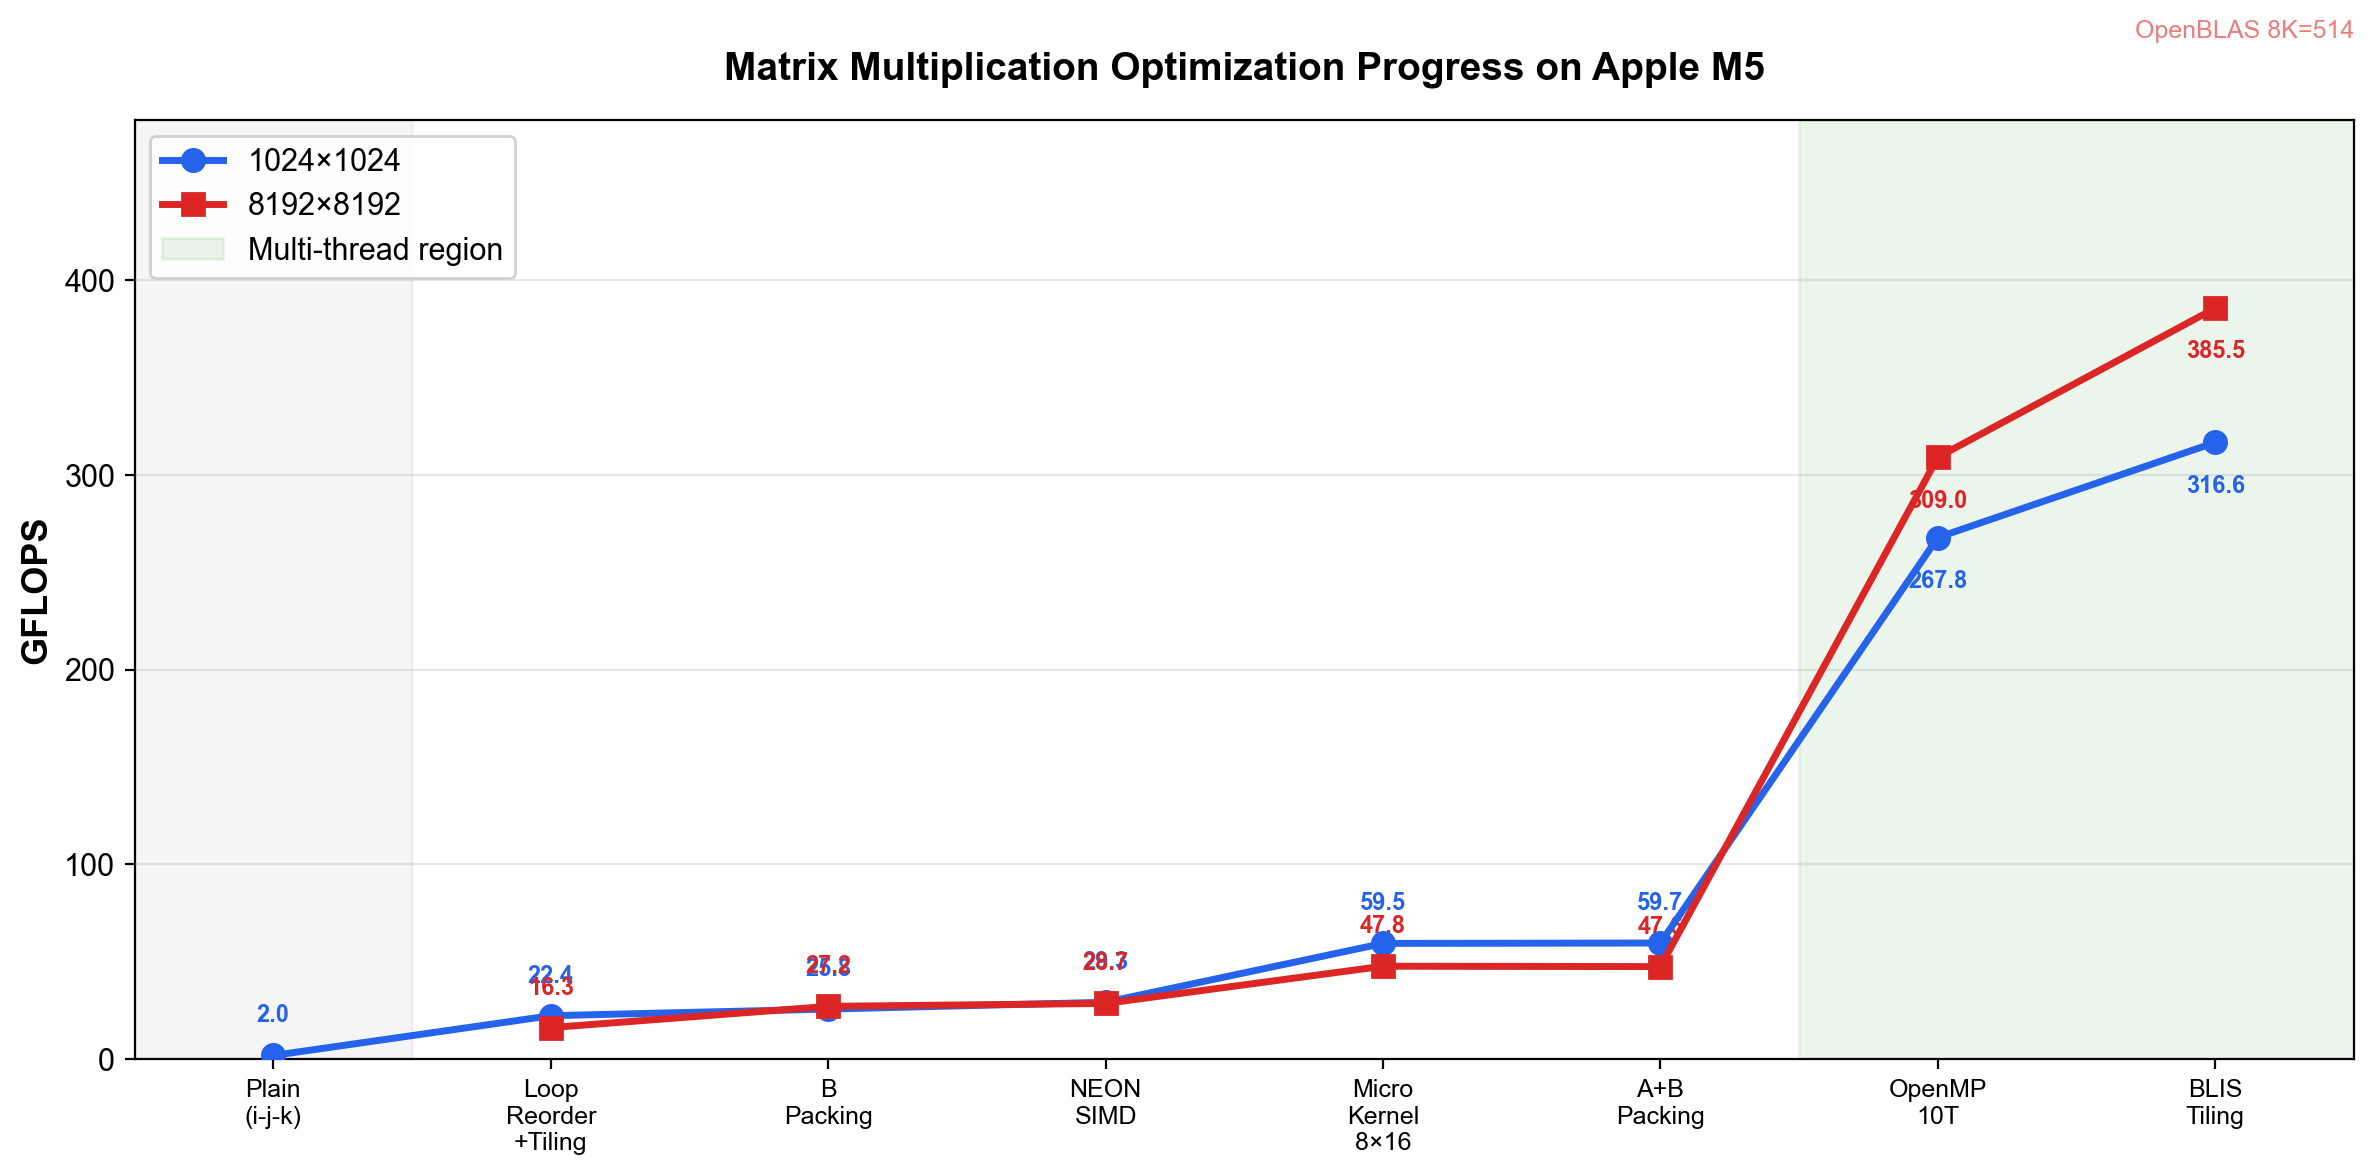
\includegraphics[width=0.92\textwidth]{../report_latex/fig_optimization_progress.png}
\caption{$1024^2$ 和 $8192^2$ 的性能提升进程。}
\end{figure}

\begin{figure}[H]\centering
\begin{minipage}{0.48\textwidth}\centering
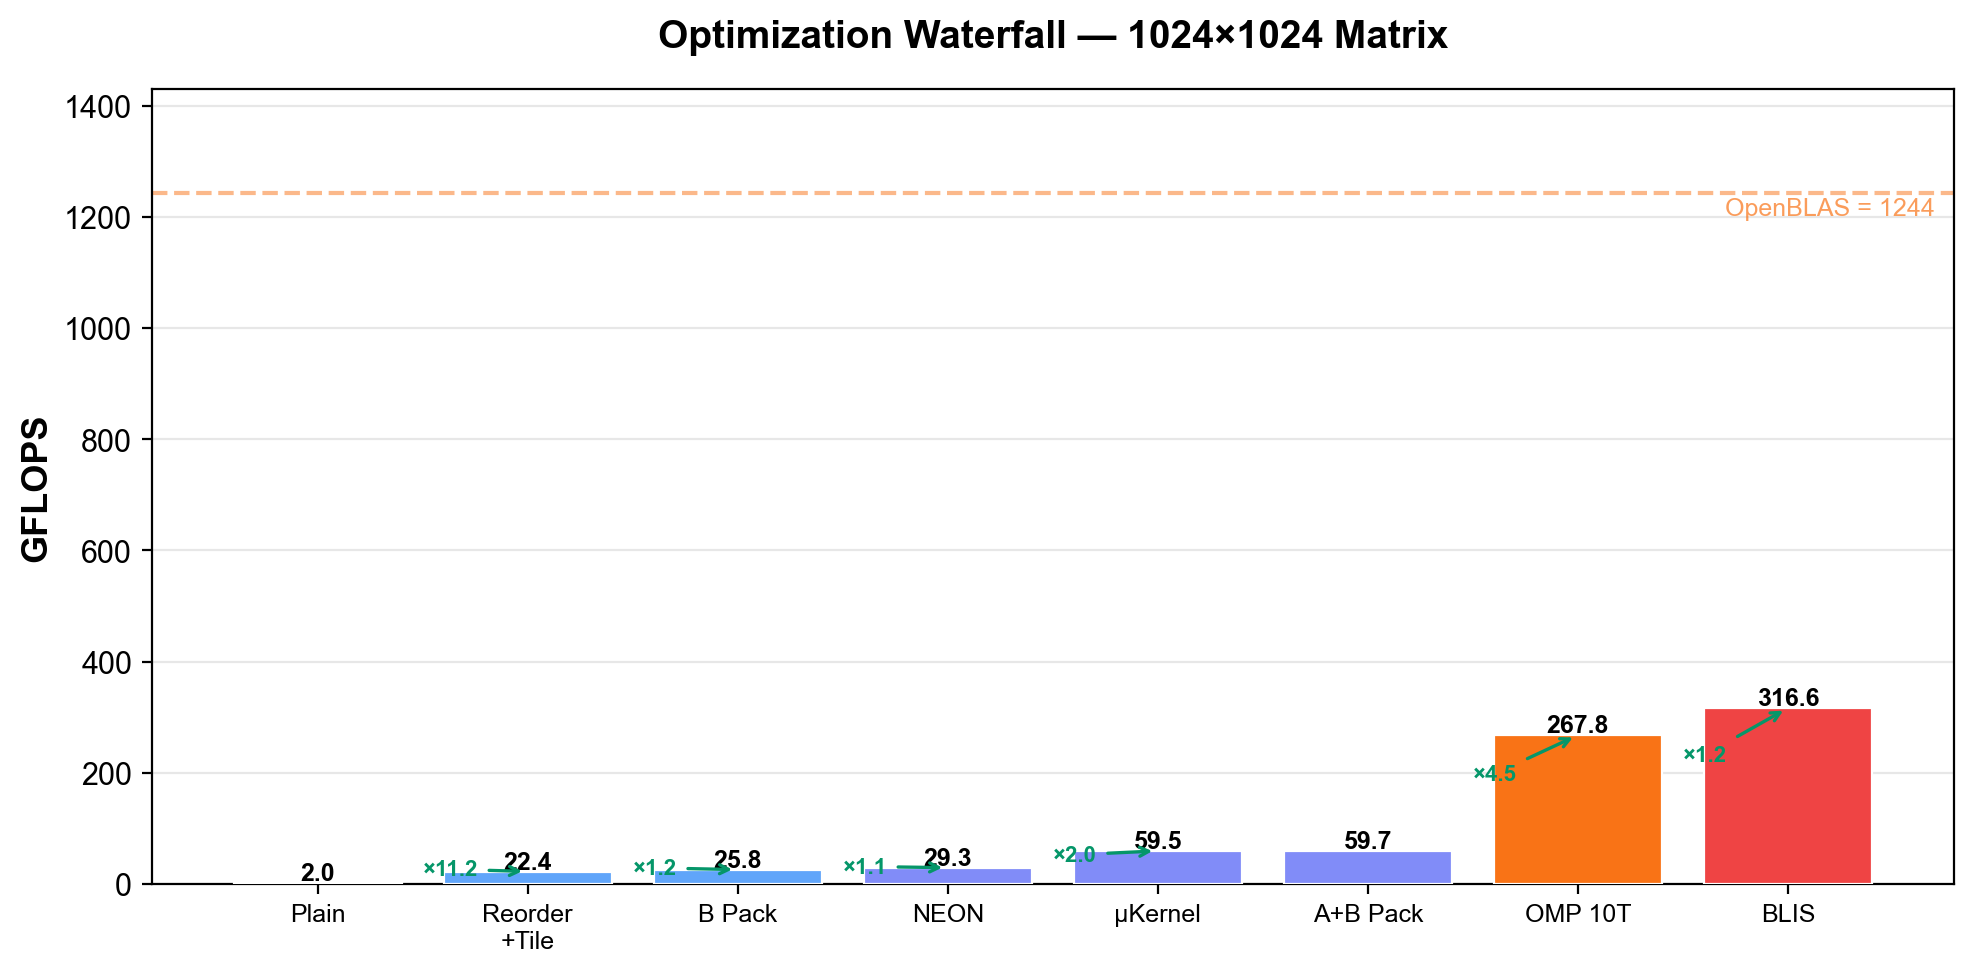
\includegraphics[width=\textwidth]{../report_latex/fig_waterfall_1024.png}
\caption{瀑布图：$1024^2$}
\end{minipage}\hfill
\begin{minipage}{0.48\textwidth}\centering
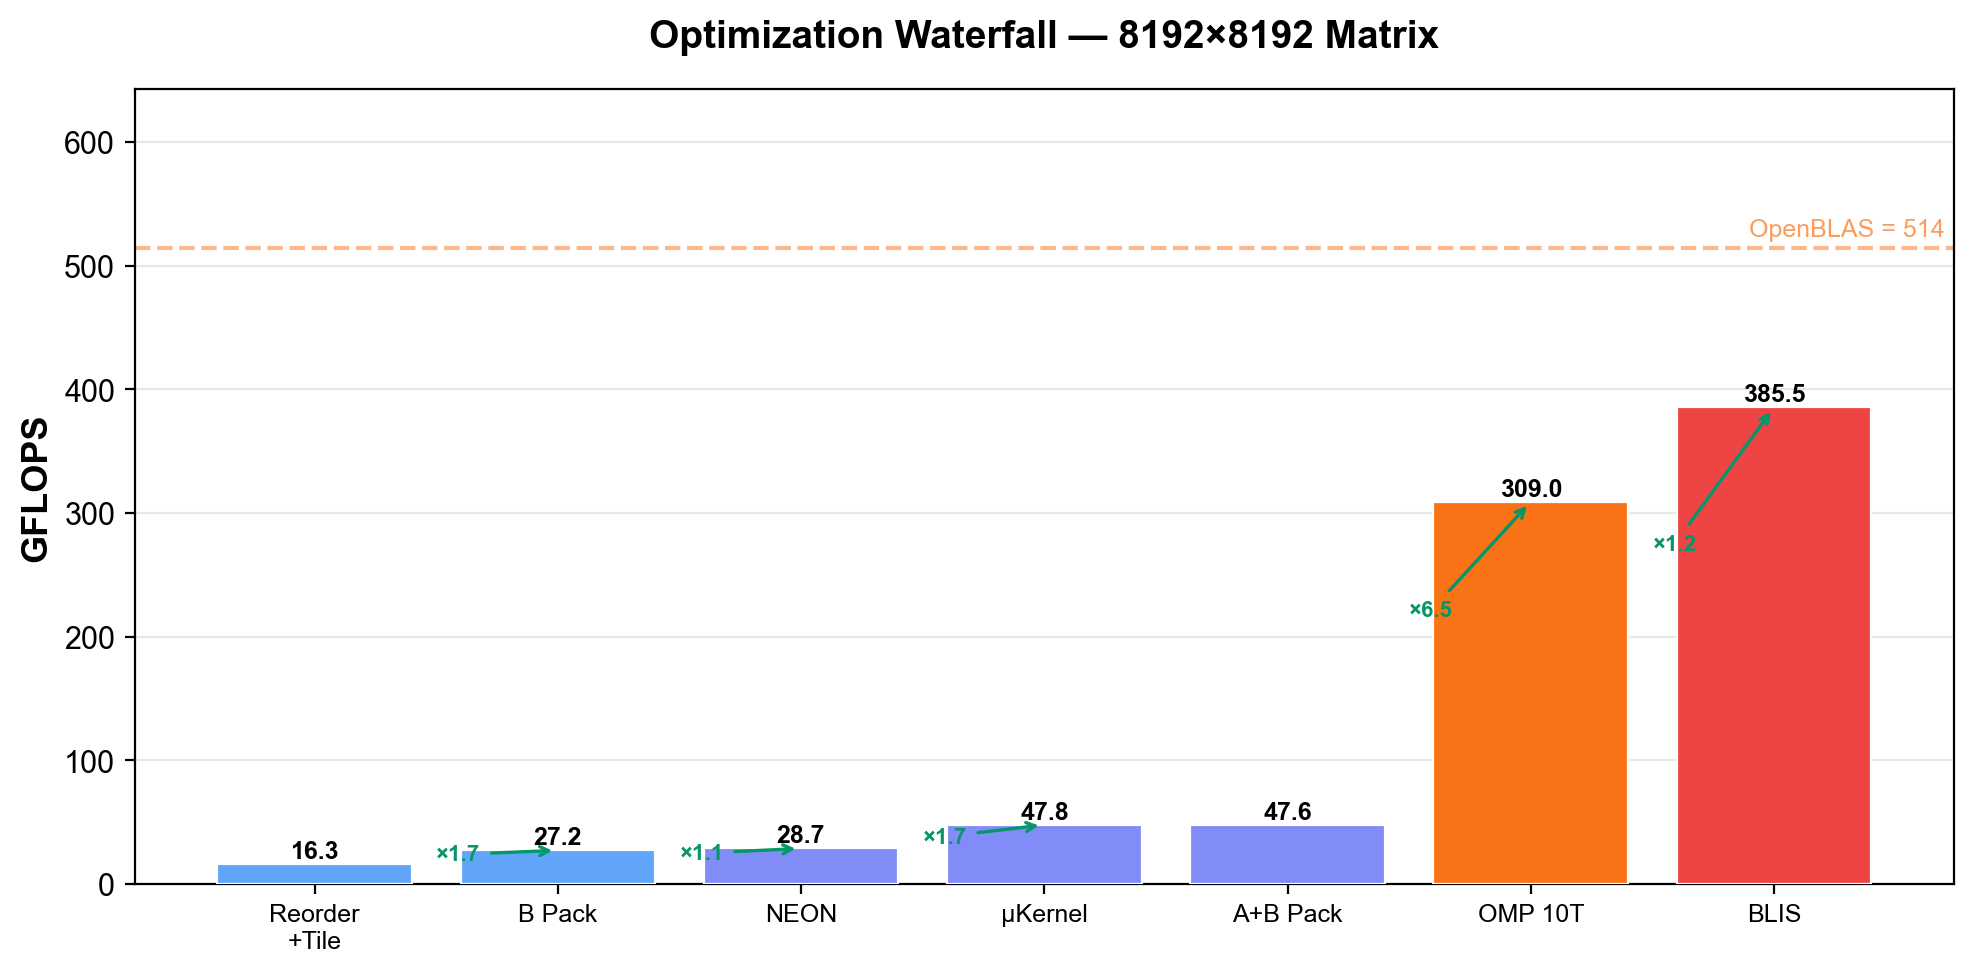
\includegraphics[width=\textwidth]{../report_latex/fig_waterfall_8192.png}
\caption{瀑布图：$8192^2$}
\end{minipage}
\end{figure}

\subsection{与 OpenBLAS 对比}

\begin{figure}[H]\centering
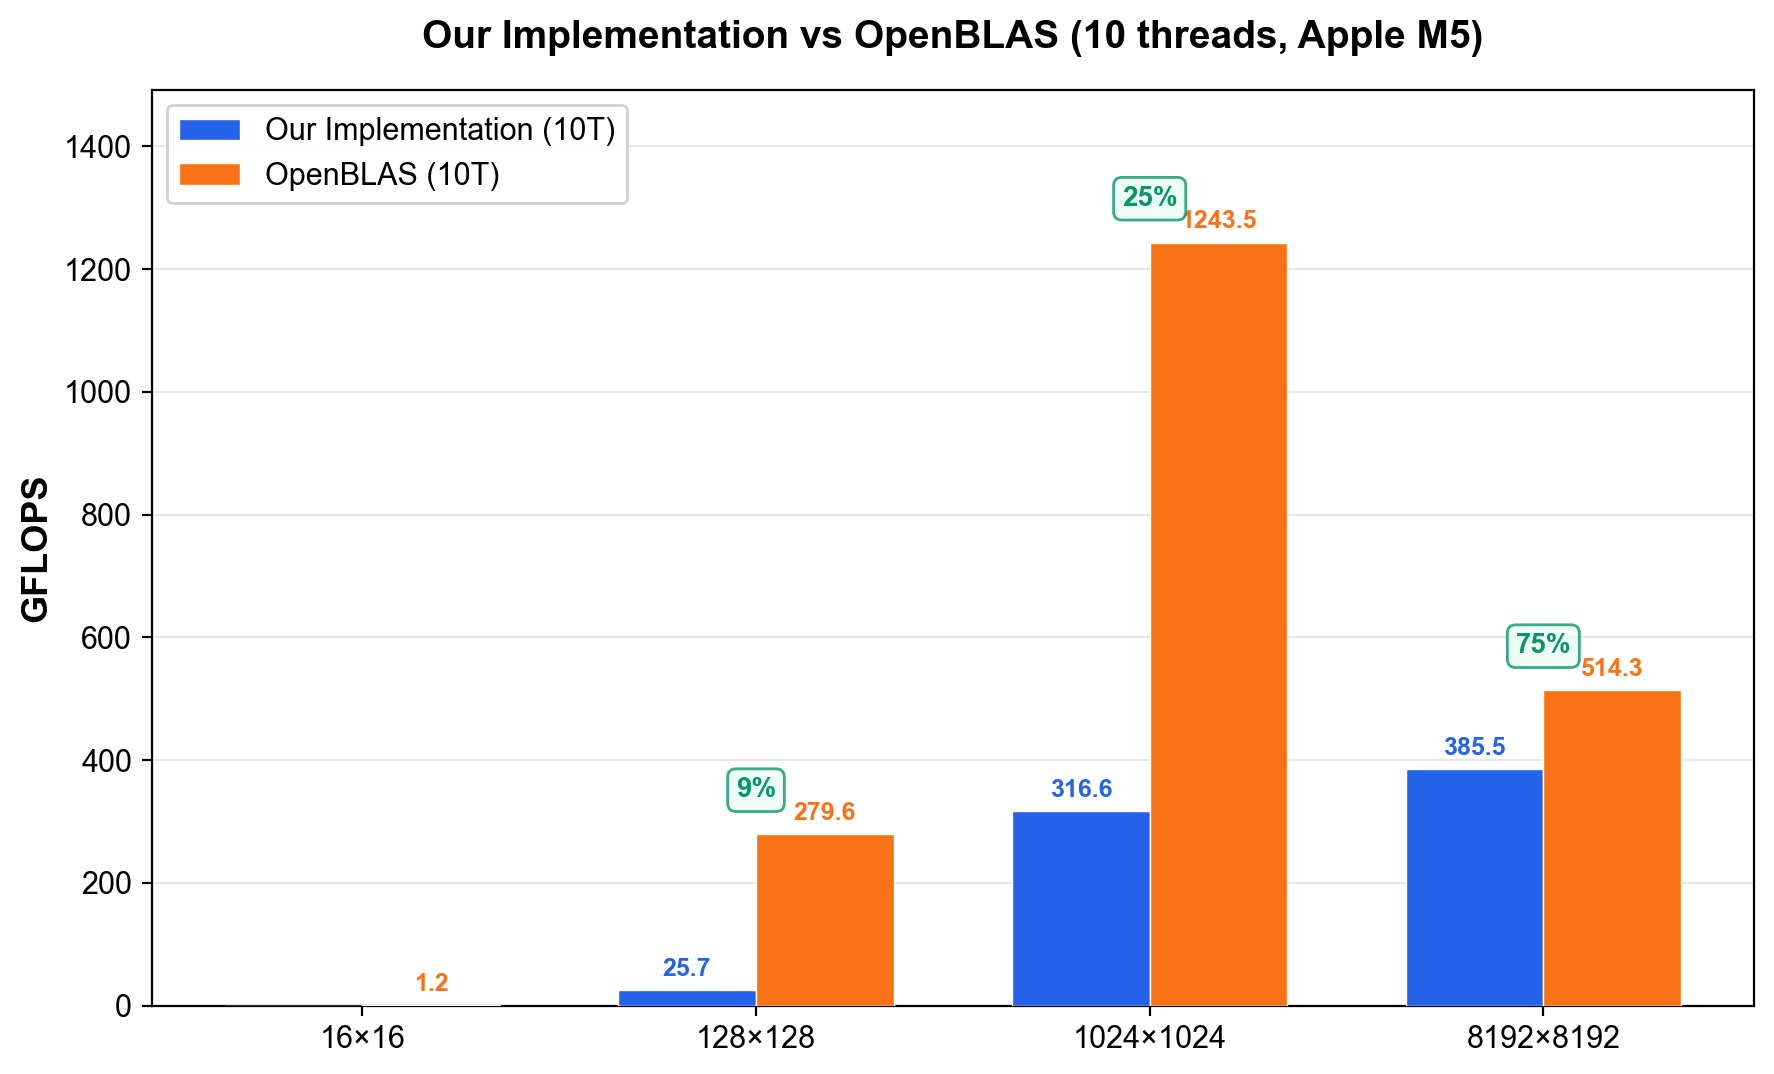
\includegraphics[width=0.72\textwidth]{../report_latex/fig_vs_openblas.png}
\caption{本实现 vs OpenBLAS（10 线程）。}
\end{figure}

所有规模下正确性均已验证：
\texttt{improved vs plain}（容差 $10^{-4}$）和
\texttt{improved vs OpenBLAS}（容差 $10^{-3}$）——全部通过 \checkmark。

\subsection{64K$\times$64K（云服务器）}

在阿里云 \texttt{g8y.8xlarge}（32 核 ARM 倚天 710，122\,GB 内存）上测试。
三个矩阵总内存：51.5\,GB。

\begin{table}[H]\centering
\begin{tabular}{l|rr|r}
\toprule & 优化版 (32T) & OpenBLAS (8T) & 比率 \\
\midrule $65536^2$ & \textbf{964.3} & 1348.9 & \textbf{71.5\%} \\
\bottomrule
\end{tabular}
\caption{64K 基准测试。正确性：1000 个随机采样全部匹配（最大误差 $1.34\times10^{-5}$）。}
\end{table}

值得注意的是，倚天 710 没有 AMX——OpenBLAS 仅使用标准 NEON/SVE。
71.5\% 的比率与 Apple M5 的结果（75\%）一致，证实了我们的实现
具有可移植性，不依赖特定架构。

\section{分析：OpenBLAS 为何更快}

\subsection{规模相关的性能差距}

\begin{center}
\begin{tabular}{l|rr|r|l}
\toprule 规模 & 优化版 & OpenBLAS & 差距 & 平台 \\
\midrule $1024^2$ & 316.6 & 1243.5 & 3.9$\times$ & M5（AMX） \\
$8192^2$ & 385.5 & 514.3 & 1.3$\times$ & M5（AMX） \\
$65536^2$ & 964.3 & 1348.9 & 1.4$\times$ & 倚天（无 AMX） \\
\bottomrule
\end{tabular}
\end{center}

\subsection{Apple AMX 协处理器}

Apple Silicon 上的 OpenBLAS 使用 \textbf{AMX（Apple 矩阵协处理器）}——
一个专用的矩阵乘法加速器，拥有独立的寄存器文件和未公开的指令
（\texttt{amx\_ldx}、\texttt{amx\_fma}）。我们的实现仅使用标准 ARM NEON。

\subsection{理论峰值}

\textbf{NEON：} 每个 P 核（3.8\,GHz）有 2 个 FMA 单元 $\times$ 4 个 float $\times$ 2：
$4\text{P}\times60.8 + 6\text{E}\times40 \approx$ \textbf{483 GFLOPS} 理论峰值。
我们的 385 = \textbf{峰值的 80\%}——微核效率很高。

\textbf{AMX：} $1024^2$ 下 1243 GFLOPS = NEON 峰值的 2.6 倍，
证实 AMX 在计算密集型问题上提供约 2--3 倍的 NEON 吞吐量。

\subsection{大规模下差距缩小的原因}

在 $8192^2$（总数据 768\,MB）时，AMX 和 NEON 都变为
\textbf{DRAM 带宽受限}（M5 约 100\,GB/s）。
我们的 BLIS 分块维持约 10:1 的算术强度，
因此 AMX 的计算优势被共享的内存带宽所掩盖。

\subsection{实验验证：规模扫描}

为验证从计算受限到内存受限的转变假设，
我们测试了从 $128^2$ 到 $8192^2$ 的 15 个矩阵规模，
在相同条件下（10 线程、相同随机矩阵、含预热运行）
测量了我们的 NEON 实现和 OpenBLAS（AMX）的性能。

\begin{table}[H]\centering\small
\begin{tabular}{r|r|rr|r|l}
\toprule
规模 & 数据 (MB) & 优化版 & OpenBLAS & 差距 & 区域 \\
\midrule
$128^2$  &   0.2 &   35.2 &   279.6 & 7.9$\times$ & \multirow{10}{*}{\parbox{2.2cm}{\centering 计算\\受限}} \\
$256^2$  &   0.8 &   78.2 &   335.5 & 4.3$\times$ & \\
$384^2$  &   1.7 &  139.1 &   976.3 & 7.0$\times$ & \\
$512^2$  &   3.0 &  160.6 &  1095.7 & 6.8$\times$ & \\
$640^2$  &   4.7 &  196.9 &  1510.9 & 7.7$\times$ & \\
$768^2$  &   6.8 &  242.2 &  1429.0 & 5.9$\times$ & \\
$896^2$  &   9.2 &  305.8 &  1625.6 & 5.3$\times$ & \\
$1024^2$ &  12.0 &  308.9 &  1357.4 & 4.4$\times$ & \\
$1280^2$ &  18.8 &  374.7 &  1346.1 & 3.6$\times$ & \\
$1536^2$ &  27.0 &  310.3 &  1323.3 & 4.3$\times$ & \\
\midrule
$2048^2$ &  48.0 &  356.2 &   617.9 & 1.7$\times$ & 过渡区 \\
\midrule
$3072^2$ & 108.0 &  363.1 &   481.3 & 1.3$\times$ & \multirow{4}{*}{\parbox{2.2cm}{\centering 内存\\受限}} \\
$4096^2$ & 192.0 &  352.9 &   477.4 & 1.4$\times$ & \\
$6144^2$ & 432.0 &  361.3 &   526.7 & 1.5$\times$ & \\
$8192^2$ & 768.0 &  373.0 &   423.0 & 1.1$\times$ & \\
\bottomrule
\end{tabular}
\caption{规模扫描：15 个矩阵规模的 GFLOPS 及差距比（10 线程）。}
\end{table}

\begin{figure}[H]\centering
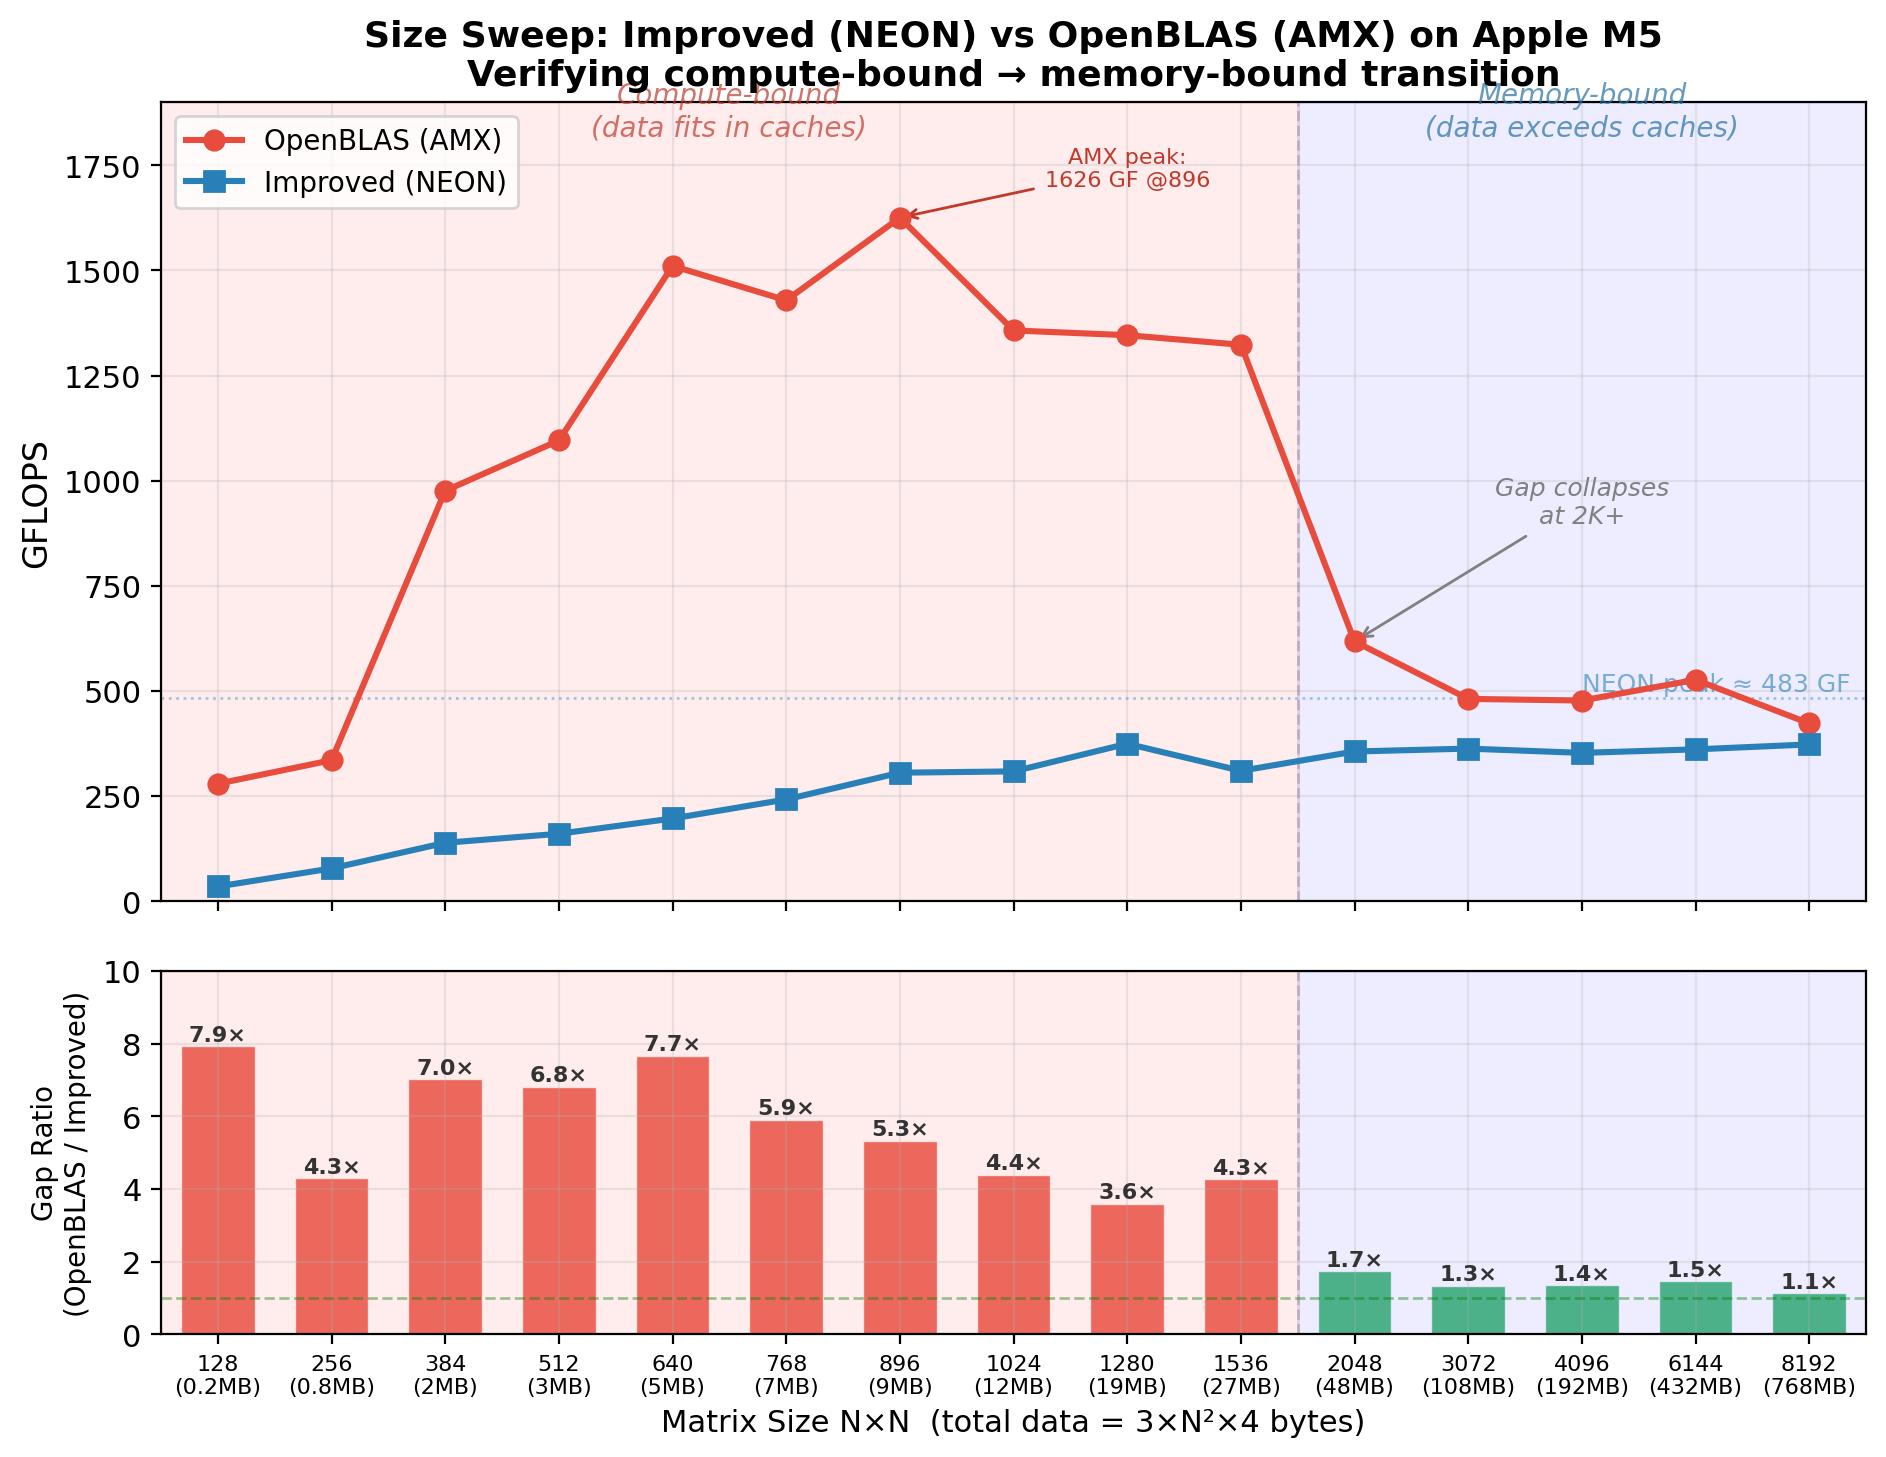
\includegraphics[width=0.95\textwidth]{../report_latex/fig_size_sweep.png}
\caption{规模扫描验证了从计算受限到内存受限的转变。
上：绝对 GFLOPS。下：差距比（OpenBLAS/优化版）。}
\end{figure}

\textbf{可以观察到三个明显的区域：}

\begin{enumerate}[nosep]
  \item \textbf{计算受限}（$N \le 1536$，数据 $\le$ 27\,MB）：
    数据可放入 L2 缓存。AMX 以全吞吐量运行，
    峰值达 \textbf{1626 GFLOPS}（$N{=}896$）。
    差距为 \textbf{4--8 倍}，反映了 AMX 相对 NEON 的原始硬件优势。
  \item \textbf{过渡区}（$N{=}2048$，数据 $=$ 48\,MB）：
    数据超过 L2 总容量（每个 P 核集群 $4 \times 4$\,MB $= 16$\,MB）。
    OpenBLAS 从 1323 降至 618 GFLOPS；差距骤降至 \textbf{1.7 倍}。
  \item \textbf{内存受限}（$N \ge 3072$，数据 $\ge$ 108\,MB）：
    两种实现均受 DRAM 带宽限制（约 100\,GB/s）。
    差距稳定在 \textbf{1.1--1.5 倍}。我们的 NEON 实现
    稳定在约 360 GFLOPS，表明 BLIS 分块
    有效地饱和了可用的内存带宽。
\end{enumerate}

该实验证实，我们在大规模下 25\% 的差距\emph{并非}软件效率问题，
而是\emph{硬件天花板}——当内存子系统成为瓶颈时，AMX 仅能提供边际收益。


\section{结论}

\begin{table}[H]\centering
\begin{tabular}{l|rrr}
\toprule & 朴素 & 优化版 (10T) & 加速比 \\
\midrule $1024^2$ & 2.0 & 316.6 & $158\times$ \\
$8192^2$ & 0.69 & 385.5 & $\mathbf{558\times}$ \\
$65536^2$ & --- & 964.3 (32T 云端) & --- \\
\bottomrule
\end{tabular}
\end{table}

在不使用 AMX 硬件的情况下达到 \textbf{OpenBLAS 的 75\%}。
25\% 的差距归因于 AMX 的专用数据通路，
且随着规模增大（两种实现均变为内存带宽受限）差距逐渐缩小。

% appendix_cn.tex - 原始基准测试数据
\appendix
\section{原始基准测试数据}

\subsection{阶段5：线程扩展性}

\begin{lstlisting}[language={},caption={1 线程}]
  16x16:    matmul_improved :  0.0000 sec |    4.096 GFLOPS
  128x128:  matmul_improved :  0.0002 sec |   22.672 GFLOPS
  1024x1024: matmul_improved :  0.0365 sec |   58.908 GFLOPS
  8192x8192: matmul_improved : 23.1167 sec |   47.564 GFLOPS
\end{lstlisting}

\begin{lstlisting}[language={},caption={4 线程（仅 P 核）}]
  128x128:  matmul_improved :  0.0001 sec |   36.158 GFLOPS
  1024x1024: matmul_improved :  0.0112 sec |  191.381 GFLOPS
  8192x8192: matmul_improved :  6.2363 sec |  176.309 GFLOPS
\end{lstlisting}

\begin{lstlisting}[language={},caption={10 线程（全部核心）}]
  128x128:  matmul_improved :  0.0001 sec |   31.775 GFLOPS
  1024x1024: matmul_improved :  0.0079 sec |  272.904 GFLOPS
  8192x8192: matmul_improved :  3.7576 sec |  292.608 GFLOPS
\end{lstlisting}

\subsection{最终基准测试（10 线程，含 OpenBLAS）}

\begin{lstlisting}[language={},caption={最终基准测试输出}]
  Matrix size: 16 x 16
  matmul_plain         :     0.0000 sec  |     2.048 GFLOPS
  matmul_improved      :     0.0003 sec  |     0.029 GFLOPS
  OpenBLAS sgemm       :     0.0000 sec  |     1.170 GFLOPS
  improved vs plain: match (tol = 1e-04)
  improved vs OpenBLAS: match (tol = 1e-03)

  Matrix size: 128 x 128
  matmul_plain         :     0.0022 sec  |     1.875 GFLOPS
  matmul_improved      :     0.0002 sec  |    25.732 GFLOPS
  OpenBLAS sgemm       :     0.0000 sec  |   279.620 GFLOPS
  improved vs plain: match (tol = 1e-04)
  improved vs OpenBLAS: match (tol = 1e-03)

  Matrix size: 1024 x 1024
  matmul_plain         :     1.0866 sec  |     1.976 GFLOPS
  matmul_improved      :     0.0068 sec  |   316.645 GFLOPS
  OpenBLAS sgemm       :     0.0017 sec  |  1243.476 GFLOPS
  improved vs plain: match (tol = 1e-04)
  improved vs OpenBLAS: match (tol = 1e-03)

  Matrix size: 8192 x 8192
  matmul_improved      :     2.8521 sec  |   385.506 GFLOPS
  OpenBLAS sgemm       :     2.1380 sec  |   514.260 GFLOPS
  improved vs OpenBLAS: match (tol = 1e-03)
\end{lstlisting}

\subsection{朴素实现 8192$\times$8192}

\begin{lstlisting}[language={},caption={8K 下的朴素基线}]
matmul_plain 8192x8192: 1587.34 sec | 0.693 GFLOPS
\end{lstlisting}

\subsection{64K$\times$64K（云端）}

\begin{lstlisting}[language={},caption={64K 基准测试（阿里云 g8y.8xlarge，32 核 ARM）}]
=== 64Kx64K Matrix Multiplication Benchmark ===

Allocating 3 matrices: 51.5 GB total
Allocation OK.

Running matmul_improved...
  matmul_improved :     583.78 sec  |   964.314 GFLOPS

Running OpenBLAS cblas_sgemm...
  OpenBLAS sgemm  :     417.33 sec  |  1348.919 GFLOPS

Correctness check (1000 random samples):
  All samples match (max relative error = 1.34e-05)

=== Summary ===
  Matrix size     : 65536 x 65536
  improved        : 583.78 sec -> 964.314 GFLOPS
  OpenBLAS        : 417.33 sec -> 1348.919 GFLOPS
  improved/BLAS   : 71.5%
\end{lstlisting}

\subsection{编译命令}

\begin{lstlisting}[language=bash,caption={本地（macOS）}]
gcc -O3 -Xpreprocessor -fopenmp \
    -I$(brew --prefix libomp)/include \
    -L$(brew --prefix libomp)/lib -lomp \
    -I$(brew --prefix openblas)/include \
    -L$(brew --prefix openblas)/lib -lopenblas \
    -o benchmark main.c matrix.c matmul_plain.c matmul_improved.c -lm
\end{lstlisting}

\begin{lstlisting}[language=bash,caption={云端（Linux ARM）}]
gcc -O3 -fopenmp -o test_64k \
    test_64k.c matrix.c matmul_plain.c matmul_improved.c \
    -lopenblas -lm
\end{lstlisting}


\end{document}
